\documentclass[12pt]{article}
\usepackage[top=1in, bottom=1in, left=1in, right=1in]{geometry}
\usepackage[justification=centering]{caption}
\usepackage{graphicx}
\usepackage{booktabs}
\usepackage{hyperref}
\usepackage{setspace}
\usepackage{cleveref}
\usepackage[version=3]{mhchem}
%\linespread{2} %double spacing

\newcommand{\p}{\textit{Paramecium}}
\newcommand{\kcl}{\ce{KCl}}
\crefformat{footnote}{#2\footnotemark[#1]#3}

\begin{document}
\title{The Effects of \ce{KCl} on \textit{Paramecium caudatum} Swimming Speed}
\author{Samuel Deslandes \and Cynthia Duque \and Roseline Idoko}
\date{\today}
\maketitle
\doublespace
\section{Introduction}
	\textit{Paramecium caudatum} is a species of unicellular organism from the phylum Ciliophora. They are commonly found in aquatic environments, especially in stagnant water bodies such as ponds or basins. As a ciliate, \p\ move using hair-like organelles which surround the outer surface of the cell called cilia. These cilia act as paddles, which move in a coordinated wave of whiplash motions to propel the \p\ through its environment.\footnote{\label{first}Summer 2016 Bio 10100 Course Supplement} Although unicellular, \p\ are large enough to be observed using a dissecting microscope.  
	
	\p, like all cells, have selectively permeable membranes which allow nonpolar solutes to diffuse through down its gradient; other (polar) solutes require the use of transmembrane proteins embedded in the lipid bilayer to transport the solute across the membrane, either down or against its gradient.\cref{first} The concentration gradient of ions inside and outside of the cell create a voltage across the cell membrane, such that the inside is slightly more negatively charged relative to the outside. ``Ions of interest with regards to the electrical charge of a typical cell may include \ce{Ca^2+},\ce{Ca^2+}, \ce{K^+}, \ce{Na^+}, \ce{Cl^-}, \ce{H^+}, \ce{Mg^2+}, \ce{NO3^-}, and \ce{NH4^+}.''\cref{first}
		 
	\ce{KCl} is a metal halide salt composed of two of the aforementioned ions. It is readily soluble in water, and is most used for making fertilizer. Other uses include forming a brine fluid for certain drilling operations\footnote{Geo Drilling Fluids inc., ``Brine Fluids Modifications 1.pdf''}, and as a sodium-free table salt alternative. These applications, especially the first two, have the potential to leech into the environment, and given its solubility also have the potential to come into contact with \p.
	
	Given that the ions that make up \ce{KCl} play a role in typical \p\ cell behavior and characteristics, and that there is a case for \kcl\ to enter the \textit{Paramecium's} typical environment, what effects may \kcl\ have on \p? Specifically, does \kcl\ decrease \p\ swimming speed? Previous experimentation suggests that this is the case, therefore it is hypothesized that \kcl\ will negatively affect the swimming speed of the \p. The null hypothesis is that \kcl\ has no effect on the swimming speed of the \p.   
	
\section{Design}
	
	To test this hypothesis, two identical electrophoresis chambers were filled with 225 mL of Dryl solution, and 4 mL of the \textit{P. caudatum} medium. 25 mL of 200 mM concentration \kcl\ solution was then added to one of the chambers, resulting in two levels of treatment: one of 0 mM \kcl\ concentration, and another of 20 mM \kcl\ concentration. The chamber used can be seen in figure \ref{chamber}\ below.
	
	
	\begin{figure}[h]
		\centering
		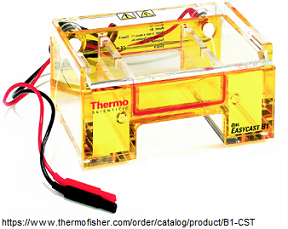
\includegraphics{chamber.png}
		\caption{Image of electrophoresis chamber used. Note: the electrodes seen above were not required for this experiment}
		\label{chamber}
	\end{figure}
	
	\noindent
	Using a millimeter grid as a reference, the distance a specimen traveled in 5 seconds was recorded by an observer. This was performed 15 times for each level of treatment. The entire experiment was performed only once. It is predicted that if we add \kcl\ to a solution containing \p\, then \p\ swimming speed will decrease.
	
	\begin{table}[h]
		\centering
		\begin{tabular}{|l|l|}
			\hline
			Variables:&\\
			\qquad Independent & \kcl\ concentration (mM) \\ \hline
			\qquad Dependent & Swimming speed (mm/s)\\ \hline
			\qquad Standardized & \quad\textbullet\ type of chamber\\ 
			& \quad\textbullet\ volume of Dryl solution (225 mL) \\
			& \quad\textbullet\ laboratory conditions \\
			& \quad\textbullet\ observer \\
			& \quad\textbullet\ observation time (5 sec)\\ \hline
			Levels of treatment & 2\\
			& \quad\textbullet\ 0 mM \kcl\ concentration \\
			& \quad\textbullet\ 20 mM \kcl\ concentration\\ \hline
			Replications & 1 \\ \hline
			Sample size & 15 \\
			\hline
		\end{tabular}
		\caption{Quick reference table of experiment design}
		\label{refTable}
	\end{table}
	
	The collected data was normalized to mm/s, and the averages of each level of treatment were calculated. A single-tailed Student's t-test was also performed to ensure statistical significance of the collected data. See the "Results" section below. 
	
\section{Results}
	A comparison of the average swimming speed of the \p\ for each treatment level can be seen in figure \ref{barGraph}. The error bars represent the standard deviation for that level of treatment. The calculated average swimming speeds were 1.07 mm/s for the 0 mM concentration solution, and 0.58 mm/s for the 20 mM concentration solution. The standard deviations were 0.404 and 0.262 respectively. \newpage
	\begin{figure}[t]
		\centering
		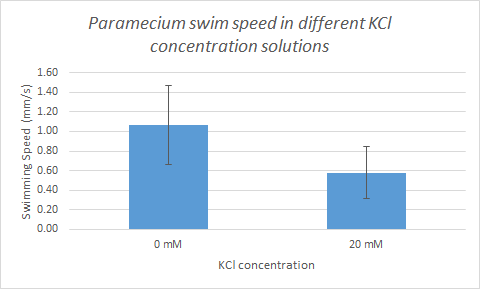
\includegraphics{chart1.png}
		\caption{Mean swimming speeds of the \p\ in 0 and 20 mM KCl concentration solutions. Error bars represent standard deviation.}
		\label{barGraph}
	\end{figure} 
	
	The results of a t-test between the swimming speeds of the specimen in the 0 mM and 20 mM \kcl\ concentration solutions can be found in table \ref{t-test} below. For a confidence level of at least 95\% with 28 degrees of freedom, the calculated t-test value must be at least 1.70. The value calculated was 3.91, which implies a confidence level exceeding 99.5\%.\\
	
	\begin{table}[h]
		\centering
		\begin{tabular}{|l|l|} \hline
			$|t-calculated|$ & 3.91 \\ \hline
			t critical for 95\% confidence level & 1.70 \\ \hline
			D.F. & 28 \\ \hline
			Confidence level & $>99.5\%$ \\ \hline
		\end{tabular}
		\caption{T-test results for the comparison between the two levels of treatment.}
		\label{t-test}
	\end{table}
	
\section{Discussion}

It was hypothesized that the presence of \kcl\ in the \p\ medium would negatively affect their swimming speed. As shown in figure \ref{barGraph}, roughly a 50\% decrease in swimming speed
was observed, supporting the alternate hypothesis. As demonstrated in table \ref{t-test}, these results are statistically significant with $>99.5\%$ probability, there for the null hypothesis is rejected, and the alternate hypothesis is truly being supported.

\subsection{Conclusion}

One possible implication of these results would be that \p\ that come into contact with \kcl\ become unable to outrun its predators, causing the population of \p\ to decrease as more
and more are eaten. \textit{Paramecium's} main predator, \textit{Didnium}, are noted as being ``voracious eaters, and will be ready to hunt for another meal after only a few hours.''\footnote{https://microbewiki.kenyon.edu/index.php/Didinium} The drop in \p\ 
population could have consequences on the carbon cycle of its ecosystem, as \p\ aid in the decomposition of plant matter. Furthermore, once \textit{Didnium's} food source (\p), becomes depleted, it 
is expected that their population will also decrease, which may have its own effects on the ecosystem. 

On the flip-side of these implications, it is also expected that with the drop in \p\ population, the population of \textit{Paramecium's} prey would increase. These include certain bacteria and in some
cases algae. One possible consequence of algae build up, for example, is the oxygen depletion of the body of water the \p\ are in, as in seen in many harmful algal blooms. 

In order to better understand the consequences of a drop in \p\ population, further experiments on the effects this change has on the ecosystem should be performed. For example, does a decrease
in the population of a \p\ species that feeds on algae lead to a large increase in algae population? Alternatively, in order to better understand the long term affects of \kcl\ on \p\, the 
swimming speed of the paramecium in both treatment levels could be measured over time. Is the retardation of the \p\ swimming speed only temporary?

\section{References}
\singlespacing
\noindent``Didinium - MicrobeWiki'', Microbewiki.kenyon.edu, 2016. [Online]. Available: \url{https://microbewiki.kenyon.edu/index.php/Didinium}. [Accessed: 15- Jun- 2016].\\

\noindent``Paramecium - Mobile Friendly'', 101science.com, 2016. [Online]. Available: \url{http://www.101science.com/paramecium.htm}. [Accessed: 15- Jun- 2016].\\

\noindent``Potassium chloride'', Wikipedia, 2016. [Online]. Available: \url{https://en.wikipedia.org/wiki/Potassium\_chloride}. [Accessed: 15- Jun- 2016].\\

\noindent ``Course Suppliment for Biological Foundations I Bio 10100'', 2016. [Book]. Department of Biology City College of New York

\end{document}